\chapter{Embedded System Design}
This chapter details the design and implementation of the embedded control system for the hydrogel bioprinter. The embedded system is responsible for coordinating the mechatronic system’s core functions, including stepper movement, memory management, bed and nozzle temperature control, and UV curing. The electronic hardware design takes the form of a custom PCB featuring an STM32F407VGT6 microcontroller, which executes the developed firmware to allow the printer to function. While more affordable alternatives exist, the STM32F407VGT6 was selected based on prior experience, thereby reducing development time and the learning curve.

The embedded system was designed to meet the following requirements, developed for the electronic design in order to allow the whole system to meet the stakeholder requirements from chapter 3:

\begin{itemize}
    \item The system must safely supply regulated 3.3 V to the logic subsystems from a 12 V DC power supply that plugs into a standard wall socket.
    \item The system must be able to drive up to five stepper motors through A4988 driver breakout modules.
    \item The system must be able to receive real-time sensor data, including extrusion force from a load cell and temperature readings from thermocouples.
    \item The device must implement switching control for a heater cartridge, Peltier module, UV curing light, and cooling fan.
    \item The system is required to receive print task via a microSD card.
    \item The printer must implement feedback control loops for extrusion pressure and temperature regulation.
    \item The system must provide headers for unused controller pins to support future upgrades.
\end{itemize}


The final assembled hydrogel bioprinter, including the implemented embedded system, is shown below in Figure~\ref{fig:FinalPrinter}:
\begin{figure}[H]
    \centering
    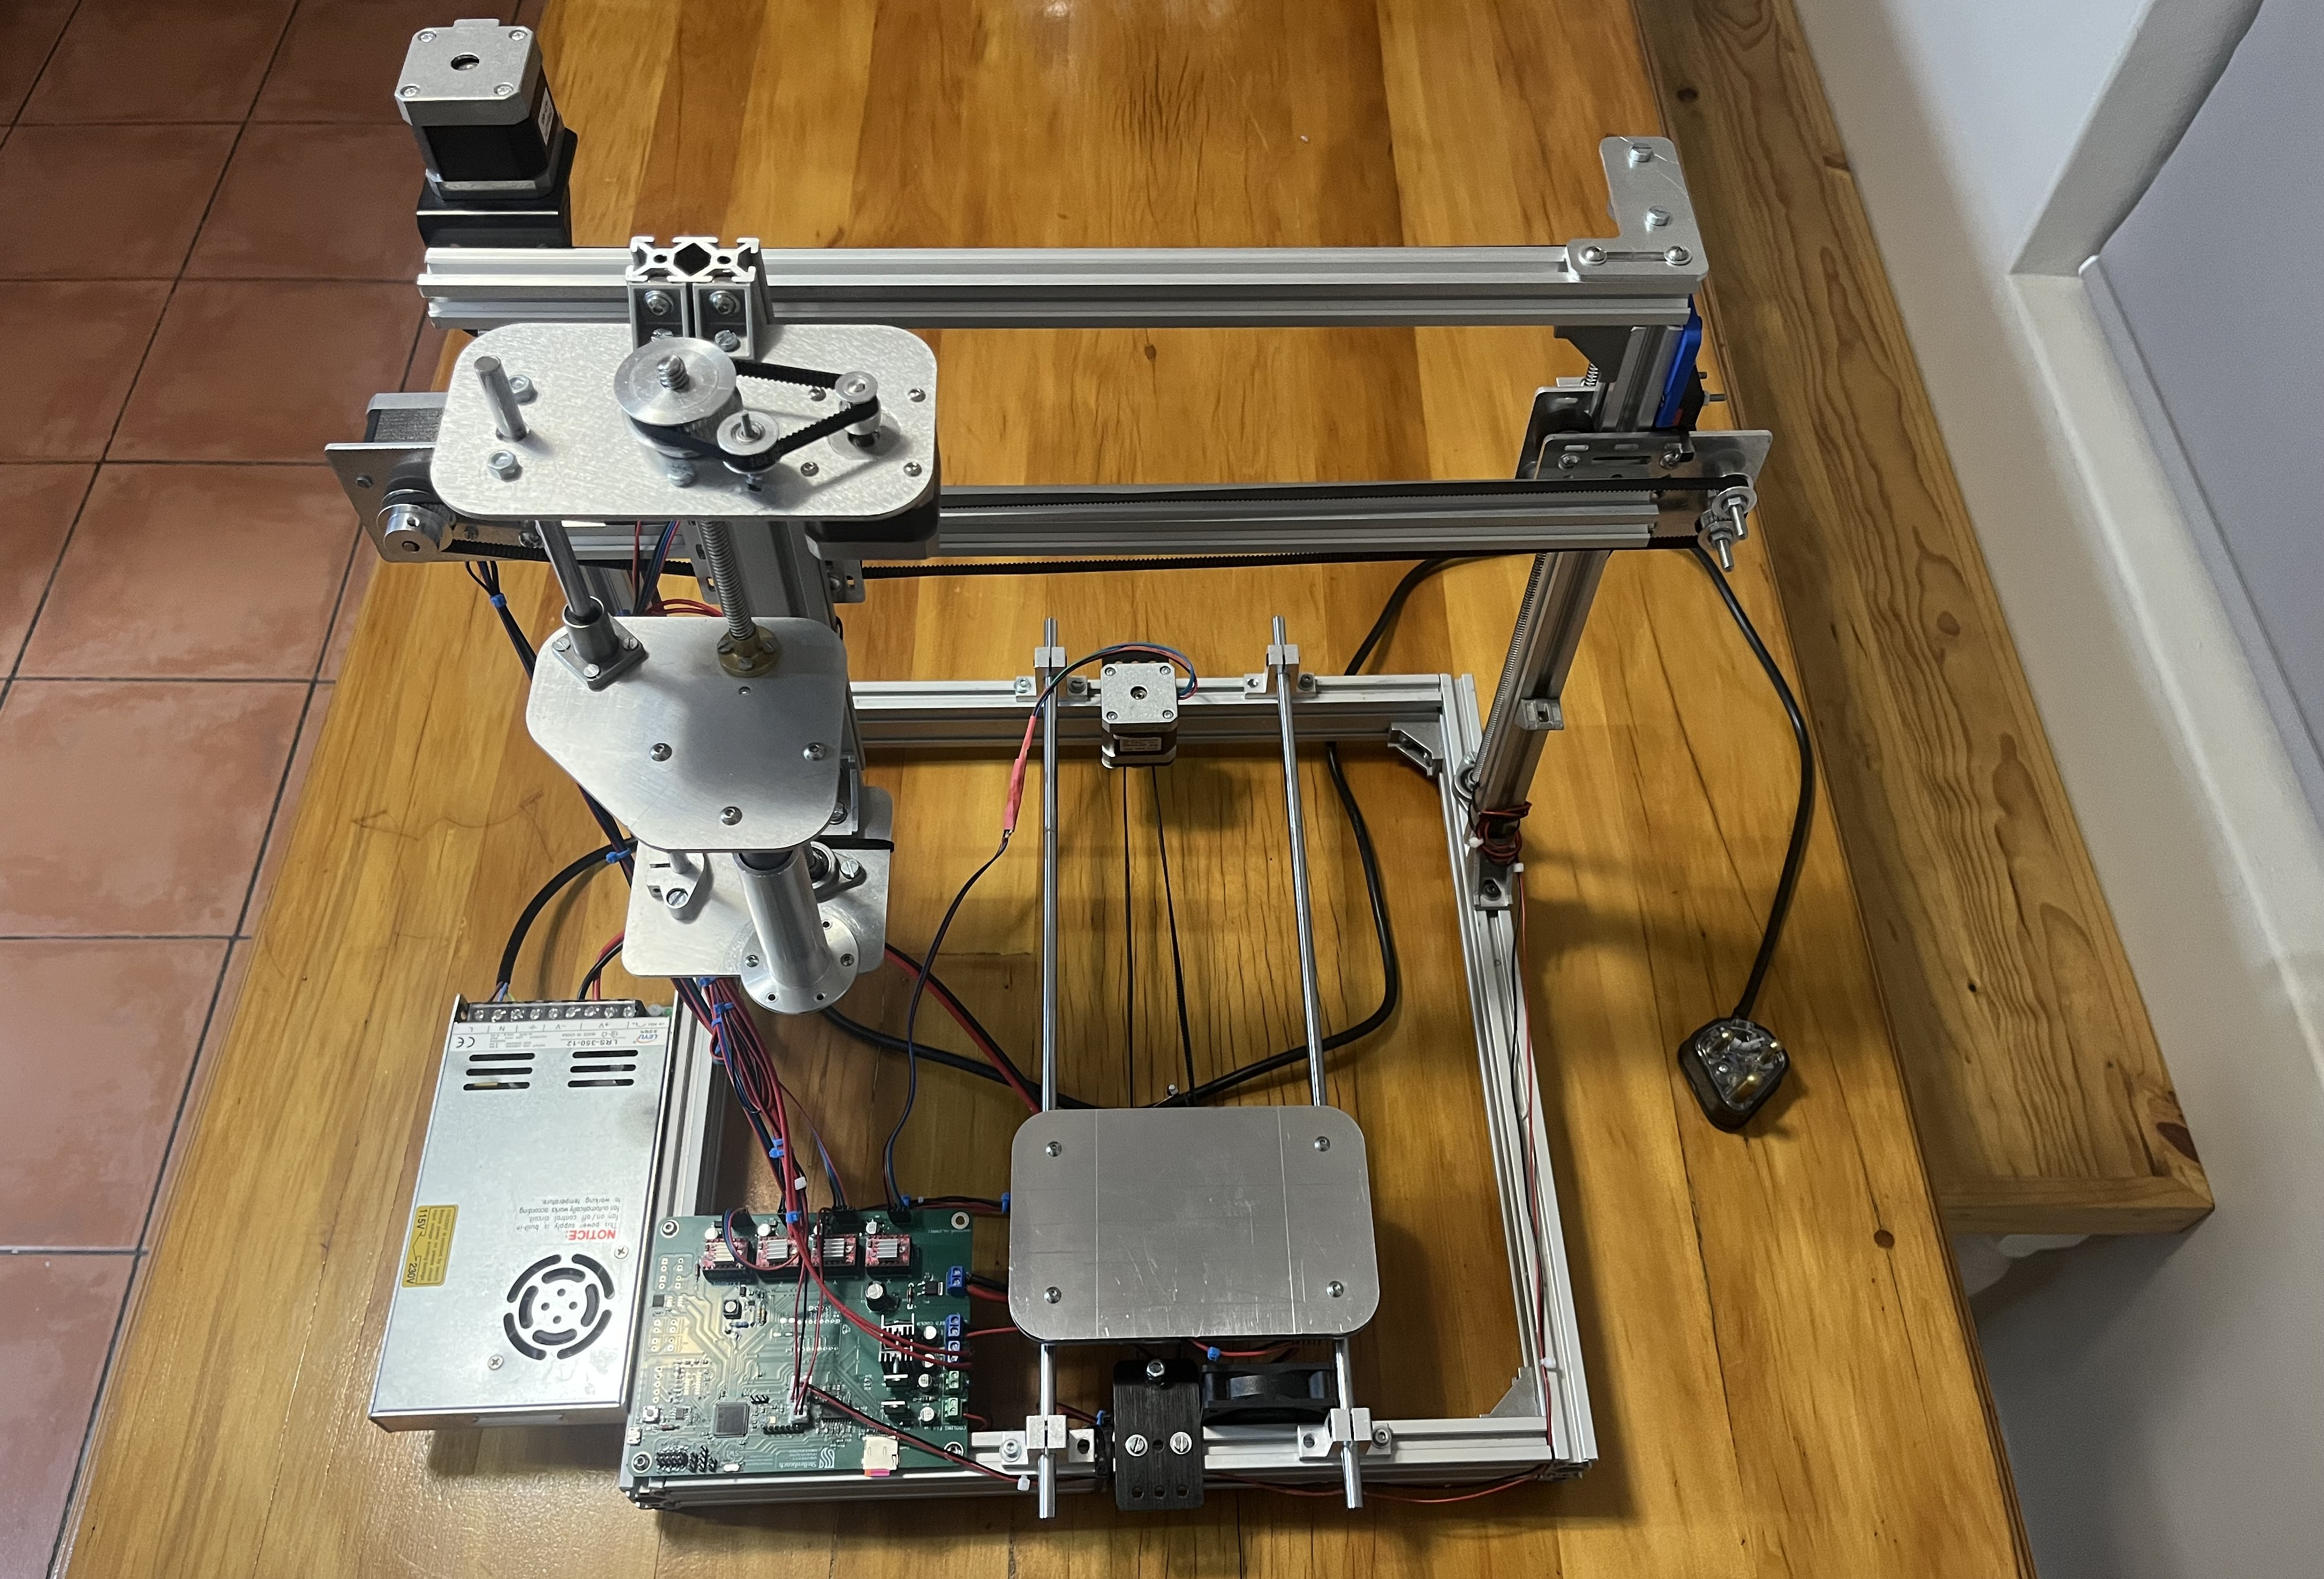
\includegraphics[scale=0.1]{figs/AssembledSystemView.jpg}
    \caption{The Final Assembled Hydrogel Bioprinter}
    \label{fig:FinalPrinter}
\end{figure}

\section{System Description}
The embedded system as a whole enables the printer's automated operation. It is powered by a 12 V PSU that directly supplies power to the stepper drivers, Peltier module, UV curing light, heater cartridge, and cooling fan. The 12 V is also converted into a regulated 3.3 V source via a buck converter to power the logic circuits. The STM32 controller reads print instructions from a microSD card so that it can then control the stepper motors (through drivers) using an ISR. During stepper operation, system information is transmitted to a laptop via a USB connection for external monitoring. External peripherals (Peltier, heater cartridge, cooling fan, and curing light) are connected to the 12 V source and switched between their ON and OFF states using N-channel power MOSFETs.

This description of the system is visually represented in the block diagram below in Figure~\ref{systemblockdiagram}. The black arrows represent the logic flow, the red arrows show the 12 V power distribution, and the green arrow shows how the 3.3 V power source is distributed.
    
\begin{figure}[H]
\centering
\begin{tikzpicture}[
  voltagecircle/.style = {circle, draw=black, thick, minimum size=1.2cm, align=center},
  block/.style = {rectangle, draw=black, thick, minimum width=3.5cm, minimum height=1cm, align=center},
  mcu/.style = {rectangle, rounded corners=5pt, draw=black, thick, minimum width=1cm, minimum height=3cm, align=center, fill=white},
  lp/.style = {rectangle, rounded corners=5pt, draw=black, thick, minimum width=1cm, minimum height=1.5cm, align=center, fill=white},
  io/.style = {rectangle, rounded corners=5pt, draw=black, thick, minimum width=2.5cm, minimum height=1cm, align=center},
  arrow/.style = {thick, -{Latex[scale=1.2]}},
  arrow2/.style = {thick, -{Latex[scale=1.2]}, color=red},
  arrow3/.style = {thick, -{Latex[scale=1.2]}, color=green}
]

% Power supply chain
\node[voltagecircle] (src) at (0.45, 8.5) {12 V\\Source};
\node[block] (reg3v3) at (5, 8.5) {3.3 V Regulator};
\node[mcu] (mcu) at (5, 4) {STM32F407\\MCU};
% Right
\node[io] (switch) at (9.2, 7.5) {Limit Switches};
\node[io] (temp) at (9.8, 6) {Temperature Sensors};
\node[io] (load) at (10, 4.5) {Extrusion Force Sensor};
\node[io] (eeprom) at (9.1, 3) {EEPROM};
\node[io] (sdcard) at (9.3, 1.5) {microSD Card};
% Left
\node[io] (step) at (0.45, 4.5) {Stepper Drivers};
\node[io] (fet) at (0, 3) {Switching MOSFETs};
% Bottom
\node[io] (usb) at (5, 1.5) {USB connection};
\node[lp] (laptop) at (0, 1.5) {Laptop};
% 12V Power flow arrows
\draw[arrow2] (src.east) -- (reg3v3.west);
\draw[arrow2] (src.south) -- (step.north);
\draw[arrow2] (0.45, 5.5) -- (-1.5, 5.5) -- (-1.5, 3.5);
% 3v3 Power flow arrows
\draw[arrow3] (reg3v3.east) -- (13,8.5) -- (13,1.5) -- (sdcard.east);
\draw[arrow3] (13,3) -- (eeprom.east);
\draw[arrow3] (13,4.5) -- (load.east);
\draw[arrow3] (13,6) -- (temp.east);
\draw[arrow3] (reg3v3.south) -- (mcu.north);
\draw[arrow3] (5,6) -- (1.5,6) -- (1.5,5);
% Logic flow arrows
\draw[arrow] (mcu.south) -- (usb.north);
\draw[arrow] (usb.west) -- (laptop.east);
\draw[arrow] (switch.west) -- (5.7,7.5) -- (5.7, 5.49);
\draw[arrow] (temp.west) -- (6.7,6) -- (6.7, 5) -- (6.2, 5);
\draw[arrow] (load.west) -- (6.2,4.5);
\draw[arrow] (eeprom.west) -- (6.25, 3);
\draw[arrow] (6.25, 3) -- (eeprom.west);
\draw[arrow] (sdcard.west) -- (6.9,1.5) -- (6.9, 2.7) -- (6.2, 2.7);
\draw[arrow] (3.77, 4.5) -- (step.east);
\draw[arrow] (3.77, 3) -- (fet.east);

\end{tikzpicture}
\caption{System Block Diagram of the Bioprinter's Embedded System}
\label{systemblockdiagram}
\end{figure}

\section{Hardware Design and Implementation}
The hardware design, as previously stated, took place in the form of a custom PCB. The PCB was designed using KiCad and manufactured by JLCPCB. The electronic system can be separated into various subsystems, including the power supply, stepper drivers, limit switches, memory handling circuit, load cell sensing circuit, temperature reading circuit, and the N-channel MOSFET switching circuit. The timing of each subsystem is coordinated by a high-speed crystal oscillator. A schematic overview of the PCB is shown in Figure~\ref{fig:pcb_overview} in Appendix C.


\subsection{Power Supply}
The power supply subsystem, shown in Figure~\ref{fig:pcb_power}, incorporates both circuit protection and voltage conversion through a buck converter. The printer is powered by a 350 W LRS PSU, which allows direct connection to a standard wall socket and converts the municipal 230 $V_{\text{RMS}}$ supply into a regulated 12 V DC output. This output is delivered to the PCB via screw terminals. 

In the event of incorrect wiring, the system makes use of reverse polarity protection using a high-side P-channel MOSFET. This ensures that, if the ground and 12 V connection are swapped, the source output is 0 V instead of -12 V. This method was chosen over a simple series diode to eliminate forward voltage drop and preserve the full 12 V for the stepper drivers and switching peripherals. 

The entire circuit board also uses bulk and decoupling capacitors to filter out a wide range of frequencies to produce stable voltage levels for both 12 V and 3.3 V components. The 12 V source also makes use of TVS diodes (SMAJ16A) positioned near inductive loads, such as the buck converter, stepper drivers, and cooling fan port, to suppress transient voltage spikes.

This subsystem also has the role of producing a stable 3.3 V source for the logic circuitry. To do this, the PCB uses an AP3211 buck converter, following the typical \SI{12}{V} to \SI{3.3}{V} application circuit by \cite{AP3211}.
\subsection{Power Debug LEDs}
The electronic hardware incorporates debug LEDs to show the presence of specific voltage levels. A green LED ($V_f \approx$\SI{2}{V}) is connected to the buck converter's 3.3 V output to confirm that the system is connected to power and that the input voltage is successfully converted to 3.3 V. A second debug LED, a blue LED ($V_f \approx$\SI{3}{V}), is connected to the USB port's 5 V pin to show when the board is connected to a laptop via USB. Both LEDs require current limiting resistors, which were calculated to limit the current to 10 mA as follows:
\begin{align*}
R_{3.3\text{V}} = \frac{3.3\ \text{V} - 2.0\ \text{V}}{10\ \text{mA}}
= 130\ \Omega
\,\,\,\,\,\,\,\,\,\,\, \text{ and } \,\,\,\,\,\,\,\,\,\,\,
R_{5\text{V}} = \frac{5.0\ \text{V} - 3.0\ \text{V}}{10\ \text{mA}}
= 200\ \Omega.
\end{align*}
For an added safety margin, \SI{220}{\ohm} resistors were used for both LEDs.

\subsection{Stepper Driver Interface}
To interface with the stepper motors, the PCB employs five A4988 driver modules, as shown in Figure~\ref{fig:pcb_steppers}. Three drivers control the motors of the 3-axis gantry, one drives the extruder stepper, and one spare driver is included to allow future upgrades, such as the addition of a second extruder. The A4988 drivers come in the form of Pololu breakout modules that plug into female headers on the PCB (visible in the 3D model in Appendix B.9). The advantage of using socketed breakout drivers is that they can be easily replaced in the event of damage. The headers follow the StepStick form factor which means the A4988 drivers can be replaced with more advanced drivers such as the TMC2209. While each driver requires a dedicated GPIO pin for its STEP and DIR inputs, to conserve controller pins, the $\overline{En}$, $\overline{SLEEP}$, $\overline{RESET}$, and the microstepping setting pins (M0, M1, and M2) are shared across all five drivers.

To limit the current, the potentiometer on each stepper driver needs to be adjusted to reach a desired reference voltage which can be obtained using the following formula: 
\[
I_{\text{limit}} \;=\; \frac{V_{\text{ref}}}{8 R_{\text{sense}}}
\qquad\Longleftrightarrow\qquad
V_{\text{ref}} \;=\; 8R_{\text{sense}}\cdot I_{\text{limit}}.
\]

By looking at the drivers and checking the stepper motor specifications, it can be concluded that:
\begin{itemize}
    \item \(R_{\text{sense}} = 0.10~\Omega\)
    \item \(I_{\text{limit}} = 1.0~\text{A}\)
\end{itemize}

\[V_{\text{ref}} \;=\; 8\cdot 0.10\cdot 1.0=0.8\text{ A.}\]

\subsection{Limit Switches}
Figure~\ref{fig:pcb_overview} shows that the circuit board provides four limit switch connection points. Only three are utilised to allow for the homing of each gantry axis. The COM pin of each limit switch is connected to ground and the NO pin is connected to a dedicated GPIO input pin (PC0-PC2) that is pulled high so that when each axis reaches the end of its range of motion, the switch gets triggered and is pulled low.
\subsection{Memory and Connectivity Interfaces}
The board employs various means of handling memory and connecting with external devices, both for reading and transmitting data as well as for programming and debugging. This functions are achieved through the inclusion of an EEPROM, a microSD port, a USB port, and an SWD interface (Figure~\ref{fig:pcb_overview}).


The controller is connected to an M24C64 EEPROM, which provides a means of storing non-volatile information via an \(I^2C\) connection, ensuring that data can be retained even after the printer’s power source is disconnected. In addition to this, the circuit board incorporates a microSD card port for reading print task files through the MCU’s SPI1 channel. A USB port is also included, allowing the board to connect to a laptop and transmit live data—such as temperature and extrusion force readings for external monitoring and analysis. Because the USB interface requires a highly accurate clock speed (48 MHz) for reliable data transmission, the PCB includes a 16 MHz external crystal oscillator to provide a precise reference for the phase-locked loop \citep{ST_STM32F405F407_datasheet}.

For programming and debugging, the board includes a 2×5 male header array. Each pin in the header is connected to the relevant system points, including the 3.3 V supply, ground, and the required STM32 pins (SWDIO, SWCLK, SWO, and NRST). During development, these SWD pins were connected to the corresponding pins of an STM32F407G-DISC1 development board to enable programming and debugging via its integrated ST-Link interface.

To improve modularity and support future upgrades, the board includes expansion headers that connect to unused MCU pins (Figure~\ref{fig:pcb_power}). These pins connect to spare GPIO, ADC, USART, \(I^2C\), and SPI channels, enabling potential additions such as external displays.

\subsection{Load Cell Circuit}
Figure~\ref{fig:pcb_sensors} shows the circuits sensor system which includes extrusion force sensing using a load cell amplifier. The amplifier circuit design was based on the SparkFun open-source HX711 load cell amplifier breakout module \citep{SparkFunHX711}. This is powered by the board's 3.3 V supply and connected to two controller GPIO pins (a clock pin and an input pin). The board has four relevant screw terminal connection points for an external load cell (RED, BLACK, WHITE, and GREEN).

The 50 kg load cell used to measure the extrusion force is configured as a half Wheatstone bridge (containing two \SI{1}{\kilo\ohm} resistors). To form a complete Wheatstone bridge, two additional \SI{1}{\kilo\ohm} resistors are required, as shown in the full load cell–to–PCB set-up in Figure~\ref{fig:loadcell}.
\begin{figure}[H]
\centering
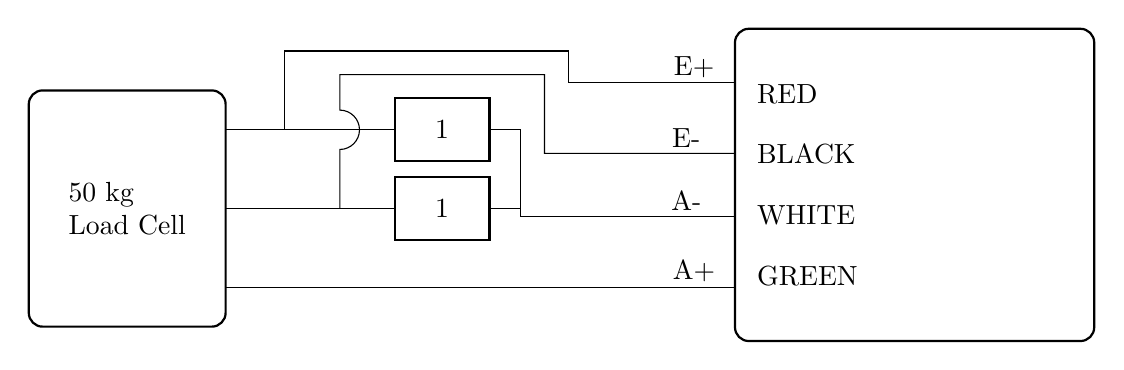
\begin{tikzpicture}[
  block/.style = {rectangle, draw=black, thick, minimum width=1.2cm, minimum height=0.8cm, align=center},
  lc/.style = {rectangle, rounded corners=5pt, draw=black, thick, minimum width=2.5cm, minimum height=3cm, align=left},
  pcb/.style = {
  rectangle, rounded corners=5pt, draw=black, thick,
  text width=4cm,            % content width
  inner xsep=8pt, inner ysep=20pt,
  align=left
  },
  arrow/.style = {thick, -{Latex[scale=1.2]}}
]

% Power supply chain
\node[lc] (loadcell) at (0, 0) {50 kg\\ Load Cell};
\node[pcb] (board) at (10,0.3) {RED \\[10pt] BLACK \\[10pt] WHITE \\[10pt] GREEN};
\node[block] (res1) at (4, 1) {\SI{1}{\kilo\ohm}};
\node[block] (res2) at (4, 0) {\SI{1}{\kilo\ohm}};
% connections
\draw (1.25,-1) -- (7.73,-1);
\draw (1.25, 0) -- (3.4,0);
\draw (1.25, 1) -- (3.4,1);
\draw (4.6, 1) -- (5,1) -- (5,-0.1) -- (7.73,-0.1);
\draw (4.6, 0) -- (5,0);
\draw (2.7,0) -- (2.7,0.75) 
      arc[start angle=-90,end angle=90,radius=0.25cm] -- (2.7,1.7) -- (5.3,1.7) -- (5.3,0.7) -- (7.73,0.7);
\draw (2,1) -- (2,2) -- (5.6,2) -- (5.6,1.6) -- (7.73,1.6);

\node at (7.2,1.8) {E+};
\node at (7.1,0.9) {E-};
\node at (7.1,0.1) {A-};
\node at (7.2,-0.8) {A+};
\end{tikzpicture}
\caption{Load Cell Setup}
\label{fig:loadcell}
\end{figure}

\subsection{Thermocouple Circuit}
The temperature sensing circuit is shown in Figure~\ref{fig:pcb_sensors}. This uses a MAX6675 K-type thermocouple, which is connected to the STM32's SPI2 pins (PB12-PB14). The amplifier receives the analogue thermocouple input, converts the signal into a digital value, and outputs this to the controller via the Serial Peripheral Interface. 

To allow the controller to read multiple thermocouples using a single amplifier, an analogue multiplexer (TMUX1208) is used. The MUX cycles through eight two-pin thermocouple screw terminals, where the T+ line connects to the amplifier input and the T– line is tied to ground. Channel selection is controlled by the MUX’s enable pin (EN) and three select pins (A0, A1, A2). The binary combination of these pins determines which of the eight thermocouple channels is connected to the amplifier input at a given time.

\subsection{FET Switching Circuit}
Figure~\ref{fig:pcb_control} shows the control circuit responsible for switching the system's various 12 V peripherals. These 12 V peripherals (each connected via two-pin screw terminals), include a Peltier cooling module, an E3D heater cartridge, a cooling fan, and a UV curing light. For safety reasons and due to the use of a non-curable surrogate gel in the experimental procedure (described in Chapter 5), a blue led was used in place of the UV light to demonstrate functionality. 

The peripherals are switched using N-Channel power MOSFETs (IRLZ44N), which are capable of handling high currents required by components such as the Peltier module (maximum current 7 A). The transistors are configured as low-side switches, with their source terminals tied to ground, drains connected to the negative side of the loads, and gates driven by STM32 GPIO outputs. If fully implemented, a UV light would be kept in a fixed position and flood the print bed with an adjustable intensity, which would be set by a duty cycle read from the microSD card during print commands.

A potential issue with this arrangement is that the transistor gates act as capacitive loads. When GPIO outputs transitions from high to low, the stored charge from the gate capacitance discharges into the MCU pin as a temporary transient discharge current. Since each GPIO pin is only rated for 25 mA \citep{ST_STM32F405F407_datasheet}, this risks damaging the controller. To mitigate this, small series resistors are placed at each gate to limit the initial discharge current.  In addition, an octal bus transceiver (SN74HC245DWR) is used as a protective buffer stage between the MCU and the MOSFET gates. This configuration not only shields the microcontroller from harmful transient currents but also improves signal integrity when driving multiple high-capacitance gates.

\subsection{PCB Design}
The embedded hardware was implemented on a custom PCB designed in KiCad and fabricated by JLCPCB. Its design required a number of engineering decisions regarding trace widths, layer count, and overall routing strategy.

The PCB is a two-layer board, with the bottom copper layer serving primarily as a ground plane and the top layer carrying power and signal routes. The complete board layout is shown in Figures~\ref{fig:pcb_3d_view} to~\ref{fig:pcb_bottom_layer}. In areas supplying the 12 V peripherals, such as the switching MOSFETs and stepper drivers, the top copper includes solid planes to provide sufficient current capacity while minimizing temperature rise.

Signal routing on the top layer generally uses 0.3 mm traces, while 3.3 V power lines were widened to 0.5 mm. The 0.5~mm trace width is justified through the empirically derived IPC-2221 current-temperature relationship, to estimate a minimum width (W) of a 1~oz/$ft^2$ thick copper trace to conduct the maximum buck-converter output current of 1.5~A with a $5~^\circ$C temperature rise:
\[
W = \frac{1}{t_{\text{cu}}}\left(\frac{I}{k(\Delta T)^{0.44}}\right)^{\frac{1}{0.725}} = \frac{1}{1.378}\left(\frac{1.5}{0.048(5)^{0.44}}\right)^{\frac{1}{0.725}} = 16.9~\text{mil} = 0.43~\text{mm}.
\]


Communication traces connecting the SD card, EEPROM, USB interface, MAX6675 thermocouple amplifier, and HX711 load cell amplifier to the STM32 microcontroller were deliberately kept short and closely routed to the MCU, with spacing between traces maximised (as far as reasonably possible) to preserve signal integrity. Similar care was taken around the buck converter circuitry to minimize interference arising from its high-frequency operation.

\section{Software Design and Implementation}
The firmware governs the 3D printer's operation. After initialising its peripherals, the system homes the gantry to its reference position and zeros the coordinate axes. It then enters an interrupt-driven routine that handles all stepper motion while the main loop cycles through system tasks such as SD card reading, USB transmission, and MOSFET duty cycle updates. The system's general software flow is visually represented in Figure~\ref{softwareflowdiagram}.

\begin{figure}[H]
\centering
\begin{tikzpicture}[
  circ/.style = {circle, draw=black, thick, minimum size=1.2cm, align=center},
  block/.style = {rectangle, draw=black, thick, minimum width=3.5cm, minimum height=1cm, align=center},
  io/.style = {rectangle, rounded corners=5pt, draw=black, thick, minimum width=2.5cm, minimum height=1cm, align=center},
  arrow/.style = {thick, -{Latex[scale=1.2]}}
]

\node[circ] (power) at (11, 5) {Power\\On};
\node[io] (sysInit) at (7.5, 5) {Initialize\\System};
\node[io] (home) at (3.5, 5) {Home};
\node[io] (zero) at (0, 5) {Zero\\Coordinates};

\node[io] (isr) at (3, 3.4) {Interrupt Service Routine};
\node[io] (step) at (8, 3.4) {Move Steppers};

\node[io] (queue) at (3, 1.7) {Add Task To\\ISR Queue};


\node[circ] (while) at (0, 0) {While\\Loop};
\node[io] (sd) at (3, 0) {Read\\SD Card};
\node[io] (fet) at (6, 0) {Update\\MOSFETs};
\node[io] (usb) at (9, 0) {USB\\Transmit};
\node[circ] (end) at (11.7, 0) {End of\\Loop};

% Logic flow arrows
\draw[arrow] (power.west) -- (sysInit.east);
\draw[arrow] (sysInit.west) -- (home.east);
\draw[arrow] (home.west) -- (zero.east);
\draw[arrow] (zero.south) -- (while.north);
\draw[arrow] (while.east) -- (sd.west);
\draw[arrow] (sd.east) -- (fet.west);
\draw[arrow] (fet.east) -- (usb.west);
\draw[arrow] (usb.east) -- (end.west);

\draw[arrow] (isr.east) -- (step.west);
\draw[arrow] (0, 3.4) -- (isr.west);

\draw[arrow] (sd.north) -- (queue.south);
\draw[arrow] (queue.north) -- (isr.south);
\end{tikzpicture}
\caption{Bioprinter's Generalised Software Flow Diagram}
\label{softwareflowdiagram}
\end{figure}

\subsection{Homing}
Upon startup, after all system peripherals have been initialised, the printer performs a homing sequence in which the gantry moves each of its three axes towards known reference positions (0, 0, 0). This procedure establishes the origin of the its coordinate system, ensuring that its absolute extruder position for a given coordinate remains consistent between power cycles.

The A4988 drivers are enabled (EN low, RESET and SLEEP high) and configured for 1/16 microstepping (M0,M1, and M2 high). Each driver's DIR pin is set so that each axis moves towards the corresponding limit switch. Each normally-open limit switch is connected to a dedicated GPIO input pin that is pulled high internally. When the limit switch closes, the input pin is connected to ground and goes low.

Step timing is handled by TIM5, which runs at 1~MHz (PSC = 83), giving a 1 µs counter tick. Each step pulse is held high for 5 µs and then low for an axis-specific duration so that each axis moves at approximately 16 mm/s. During homing, only one axis moves at a time until its limit switch GPIO input is no longer high, at which point that axis stops and the next axis begins. The axes are homed in the order of Z, Y, and lastly X.

\subsection{Stepper Logic}
After the gantry is homed, the printer's motion system is scheduled through an interrupt service routine (ISR). The advantage of timing the stepper movements with scheduled interrupts, rather than triggering each step from within the program’s \texttt{while(1)} loop, is that step pulses are consistently generated on time and remain unaffected by lower-priority tasks that could introduce delays. Although the firmware may not currently be performing computationally intensive operations that make this approach strictly necessary, it provides future-proofing by ensuring reliable motion control even as more time-demanding features (G-code parsing) are added.

Once the system is homed, the enable pin is set low, and the sleep and reset pins are set high as instructed by \cite{Allegro_A4988}. The microstep selection pins are all driven high to configure the driver for 1/16 microstepping mode, ensuring maximum positional accuracy for the belt-driven axes. The DIR pins for each driver are pre-defined in the code as high or low to define each axis' positive direction. Before the ISR starts executing the commands from the SD card, the stepper coordinates are set to zero with the command \texttt{Stepper\_ResetPosition(x0, y0, z0, e0)}.

\begin{figure}[H]
\centering
\begin{tikzpicture}[
  circ/.style = {circle, draw=black, thick, minimum size=1.2cm, align=center},
  block/.style = {rectangle, draw=black, thick, minimum width=3.5cm, minimum height=1cm, align=center},
  io/.style = {rectangle, rounded corners=5pt, draw=black, thick, minimum width=2.5cm, minimum height=1cm, align=center},
  arrow/.style = {thick, -{Latex[scale=1.2]}}
]
\node[circ] (init) at (11.5, 6.5) {Start ISR\\Segment};
\node[io] (calc) at (8.25, 6.5) {Calculate \\$N_x\,\text{and}\,N_\text{max}$};
\node[io] (reset) at (4.2, 6.5) {Reset accumulators\\($i=0\,\text{and}\,e_x=0$)};
\node[io] (dir) at (0, 6.5) {Set $\text{DIR}_x$};

\node[io] (queue) at (3, 5) {Start the next ISR\\segment in the queue};
\node (true1) at (2.2,4) {TRUE};
\node[circ] (interrupt) at (0, 3) {Interrupt\\Triggered};
\node[io] (comp1) at (3, 3) {$i \ge N_{\max}$};
\node (false1) at (5.1,3.3) {FALSE};

\node[io] (comp2) at (11, 3) {$e_x \ge N_{\max}$};
\node[io] (step) at (11, 1) {Generate\\step pulse};
\node[io] (sub) at (7, 1) {$e_x \leftarrow e_x - N_{\max}$};
\node[io] (wait) at (3, 0) {Wait for\\next interrupt};
\node (true2) at (10.3,2.2) {TRUE};
\node (false2) at (10.3,-0.3) {FALSE};
\node[io] (accum) at (7.5,3)
  {$\begin{aligned}
      e_x &\leftarrow e_x + N_x\\
      i   &\leftarrow i + 1
    \end{aligned}$};
% Logic flow arrows
\draw[arrow] (init.west) -- (calc.east);
\draw[arrow] (calc.west) -- (reset.east);
\draw[arrow] (reset.west) -- (dir.east);
\draw[arrow] (dir.south) -- (interrupt.north);
\draw[arrow] (interrupt.east) -- (comp1.west);
\draw[arrow] (comp1.north) -- (queue.south);
\draw[arrow] (comp1.east) -- (accum.west);
\draw[arrow] (accum.east) -- (comp2.west);
\draw[arrow] (comp2.south) -- (step.north);
\draw[arrow] (step.west) -- (sub.east);
\draw[arrow] (sub.west) -- (3,1) -- (wait.north);
\draw[arrow] (wait.west) -- (0,0) -- (interrupt.south);
\draw[arrow] (comp2.east) -- (12.5,3) -- (12.5,0) -- (wait.east);

\end{tikzpicture}
\caption{Software Diagram of an ISR Segment on the X-axis}
\label{isrdiagram}
\end{figure}

The ISR, driven by TIM1, implements motion commands executed from a circular queue. The commands use the format of x position, y position, z position, speed, extrusion rate, and a boolean input that determines whether the command is implemented according to a relative (1) or absolute (0) coordinate system. From this, the ISR operates with the following steps (shown in Figure~\ref{isrdiagram}):
\begin{itemize}
    \item The relative distance each axis must move is calculated (i.e. $\Delta x=x_{target}-x_{current}$).
    
    \item Using the steps per millimeter for each stepper, the required number of steps is determined (i.e. $N_x=|\Delta x \times \text{STEPS\_PER\_MM}| $).

    \item The direction level (DIR) is determined for each driver by considering the sign of each axis' position change and the positive direction level defined in the code.

    \item To determine the total execution time of each command, the travel length is calculated ($L=\sqrt{\Delta x^2+\Delta y^2+\Delta z^2}$), and the total time is then obtained by dividing this length by the gantry speed ($T=\frac{L}{v}$).

    \item To ensure that all axes arrive simultaneously, the maximum step count is calculated as $N_{max}=\text{max}(N_x,N_y,N_z,N_e)$.

    \item From this, the ISR runs at a frequency of $f_{\text{step}}=\frac{N_{\text{max}}}{T}$, and the interrupt period is the reciprocal.

    \item At each interrupt period, each axis increments its own Bresenham accumulator to determine whether a pulse must be generated for any of the drivers. For example, the x axis accumulator, $e_x$, increments by $N_x$ during each interrupt, but a step pulse is only generated for the x axis once $e_x\ge N_\text{max}$, in which case the accumulator will also be reduced by $N_\text{max}$.
\end{itemize}



\subsection{USB Communication}
The STM32 controller uses a USB Full-Speed CDC virtual COM port on PA11 and PA12 using the STM32 USB Device library. Upon startup, the USB system is initialised and a 1 Hz task transmits a message to communicate system information (such as temperature) via \texttt{CDC\_Transmit\_FS()}. The transmission is sent in the following format:
\begin{quote}\ttfamily
setNozTemp=30.00C, NozTemp=26.12C, Load=5.71 kg \textbackslash n
\end{quote}
A laptop can connect to the PCB via a USB cable and view the stream using any serial terminal (such as Termite), or transform the data in MATLAB during the printer's operation. The RX callback is set up but is not utilized. This introduces the opportunity for later firmware upgrades to allow the possibility of external commands being sent from a laptop for additional control. 

\subsection{SD Card Reading}
The printer reads motion commands from an SD card using the FatFs middleware over SPI communication (SPI1). Once FatFs is initialized and the file system is mounted, a command file, \texttt{PrintTask.csv}, is opened read with the \texttt{f\_open()} function.

During printer operation, the next commands (if the ISR queue has space) are read in the program's \texttt{while(1)} loop every 50~ms (20~Hz)task. The format of each command line in the CSV file is:
\[
X,\;Y,\;Z,\;\text{Speed},\;\text{ExtrusionRate},\;\text{Mode},\;\text{NozzleTemp},
\]
where \texttt{Mode} selects absolute (\texttt{0}) or relative (\texttt{1}) moves. Read command lines are queued into the ISR via \texttt{Stepper\_QueueAbs()} or \texttt{Stepper\_QueueRel()}.

\subsection{Switching Logic}
The printer switches its 12~V peripherals (nozzle heater, cooling fan, UV LED, and Peltier module) by controlling the logic levels of the gate terminals of their N-channel MOSFETs via the microcontroller. Upon startup, the Peltier gate (PB4) is driven high, keeping the cooler continuously on. The remaining three loads, are controlled via PWM through the STM32's timer channels:
\begin{itemize}
  \item Nozzle heater: \texttt{TIM3\_CH2} on \texttt{PB5}
  \item Fan: \texttt{TIM4\_CH1} on \texttt{PB6}
  \item UV LED: \texttt{TIM4\_CH2} on \texttt{PB7}
\end{itemize}
With $\text{PSC}=0$ and $\text{ARR}=4199$, each pulse width modulation channel operates at 20 kHz:
\begin{align*}
    f_\text{PWM} = \frac{f_\text{timer}}{(\text{PSC}+1)(\text{ARR}+1)} = \frac{84\text{ MHz}}{(\text{0}+1)(4199+1)} = 20\text{ kHz}.
\end{align*}
Duty cycles (0-100 \%) are updated in the \texttt{while(1)} loop every 50~ms by adjusting the channel compare register (CCR):
\begin{equation*}
 \mathrm{CCR} = \frac{\text{Duty Cycle}}{100}\,\mathrm{ARR}.
\end{equation*}
The blue LED undergoes a linear brightness modulation over a 10-second periodic interval (to show curing intensity adjustment capabilities) and the fan is set to operate at full intensity ($D=100\%$).

\section{Measurements and Results}
To verify nozzle heating and bed cooling, a FLIR ONE Pro camera captured the temperature distribution of both components (100\% duty cycle) after 10 minutes of operation, as shown in Figures~\ref{fig:nozdist} and~\ref{fig:beddist}. Due to an unavailability of hand-held thermocouple's in the M\&M Workshop during testing, a CASTALWARE digital thermometer was used to determine less accurate settling temperatures. By resting the end of the thermometer on the bed's centre, a minimum of $13~^\circ$C was recorded, and placing the probe in the E3D heater block's thermistor hole indicated a maximum of $230~^\circ$C.


\begin{figure}[H]
    \centering
    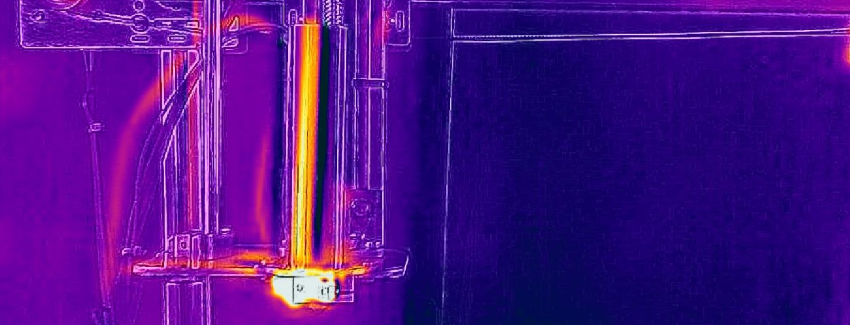
\includegraphics[scale=0.4]{figs/NozTempDistribution.png}
    \caption{Nozzle temperature distribution after 10 minutes of being active (100\% duty cycle)}
    \label{fig:nozdist}
\end{figure}


\begin{figure}[H]
    \centering
    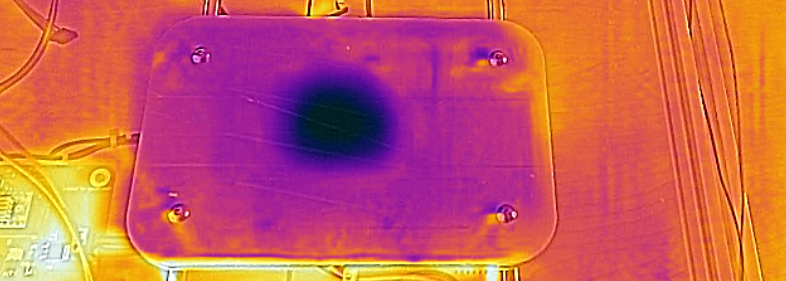
\includegraphics[scale=0.42]{figs/BedTempDist.png}
    \caption{Bed temperature distribution after 10 minutes of being active }
    \label{fig:beddist}
\end{figure}